\documentclass[border=8pt]{standalone}
\usepackage[T1]{fontenc}
\usepackage{lmodern,amsmath,amssymb,xcolor,tikz}
\usetikzlibrary{arrows.meta,calc,decorations.markings}
\definecolor{ink}{RGB}{40,45,50}
\tikzset{vertex/.style={circle,fill=ink,inner sep=1.7pt},
 resistor/.style={draw,fill=white,minimum width=5mm,minimum height=1.7mm,inner sep=0pt,sloped},
 wire/.style={line width=.8pt,postaction={decorate},decoration={markings,mark=at position .81 with {\arrow{Stealth[length=1.5mm]}}}},
 active wire/.style={wire,draw=black,line width=1.3pt},
 moveArrow/.style={draw=black,line width=1pt,-{Stealth[length=2.2mm]}},
 lab/.style={font=\normalsize,fill=white,inner sep=2pt},
 title/.style={text=black,font=\large}}
% #1 panel prefix; #2 start label; #3 next label; #4 source label.
\newcommand{\fanpanel}[4]{%
 \coordinate (#1a) at (0,0);\coordinate (#1b) at (1.5,0);
 \coordinate (#1c) at (4.1,0);\coordinate (#1d) at (5.6,0);\coordinate (#1w) at (2.8,-2.4);
 \node[vertex,label=above:$#2$] at (#1a) {};
 \node[vertex,label=above:$#3$] at (#1b) {};
 \node[vertex,label=above:$n$] at (#1c) {};
 \node[vertex,label=above:$n+1$] at (#1d) {};
 \node[vertex,label=below:$n+2$] at (#1w) {};
 \draw[active wire] (#1a)--node[resistor]{}(#1b);
 \draw[wire] (#1b)--(2.05,0);\node at (2.8,0) {$\cdots$};\draw[wire] (3.45,0)--(#1c);
 \draw[wire] (#1c)--node[resistor]{}(#1d);
 \draw[active wire] (#1a)--node[resistor]{}(#1w);
 \draw[active wire] (#1b)--node[resistor]{}(#1w);
 \draw[wire] (#1c)--node[resistor]{}(#1w);
 \draw[wire] (#1d)--node[resistor]{}(#1w);
 \node[lab,text=black,anchor=east] at (-.25,-.6) {$#4$};
 \draw[draw=black,dashed,-{Stealth[length=1.6mm]}] (-.22,-.55)--(-.025,-.075);
}
% The manuscript places live \eqref links in the three reserved label spaces.
\begin{document}
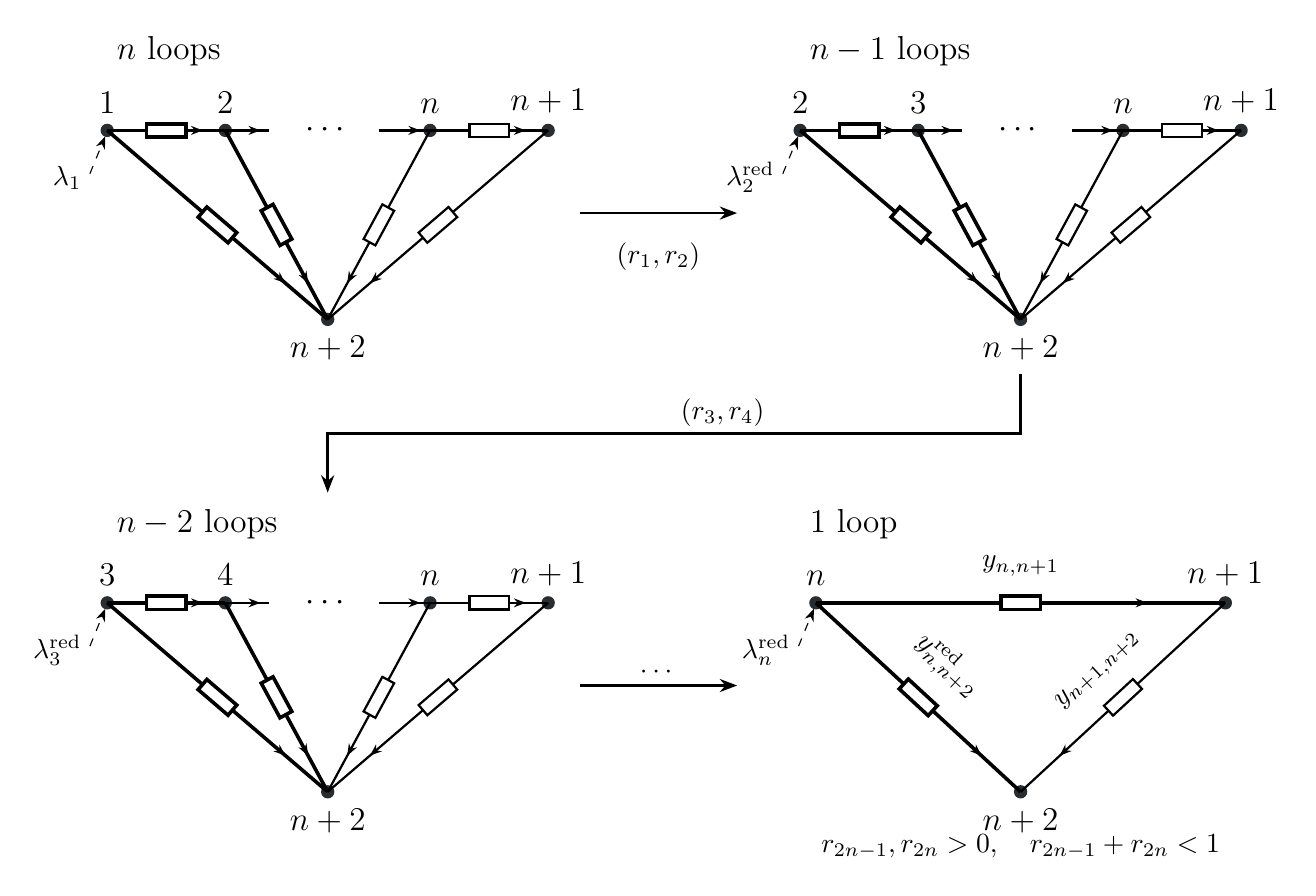
\begin{tikzpicture}[font=\large,text=black]
\begin{scope}[shift={(0,0)}]
 \node[title,anchor=west] at (0,1) {$n$ loops};
 \fanpanel{a}{1}{2}{\lambda_1}
\end{scope}
\draw[moveArrow] (6,-1.05)--node[lab,above,text=black]{\phantom{(0.00)}}(8,-1.05);
\node[text=black,font=\normalsize] at (7,-1.6) {$(r_1,r_2)$};
\begin{scope}[shift={(8.8,0)}]
 \node[title,anchor=west] at (0,1) {$n-1$ loops};
 \fanpanel{b}{2}{3}{\lambda_2^{\mathrm{red}}}
\end{scope}
\draw[moveArrow] (11.6,-3.1)--(11.6,-3.85)--node[lab,above,text=black]{\phantom{(0.00),} $\ (r_3,r_4)$}(2.8,-3.85)--(2.8,-4.6);

\begin{scope}[shift={(0,-6)}]
 \node[title,anchor=west] at (0,1) {$n-2$ loops};
 \fanpanel{c}{3}{4}{\lambda_3^{\mathrm{red}}}
\end{scope}
\draw[moveArrow] (6,-7.05)--node[lab,above,text=black]{$\cdots$}(8,-7.05);
\node[text=black,font=\normalsize] at (7,-7.6) {\phantom{(0.00)}};
\begin{scope}[shift={(8.8,-6)}]
 \node[title,anchor=west] at (0,1) {$1$ loop};
 \coordinate (dn) at (.2,0);\coordinate (dp) at (5.4,0);\coordinate (dw) at (2.8,-2.4);
 \node[vertex,label=above:$n$] at (dn) {};\node[vertex,label=above:$n+1$] at (dp) {};\node[vertex,label=below:$n+2$] at (dw) {};
 \draw[active wire] (dn)--node[resistor]{}node[lab,above=2.5mm]{$y_{n,n+1}$}(dp);
 \draw[active wire] (dn)--node[resistor]{}node[lab,sloped,above=2.5mm]{$y_{n,n+2}^{\mathrm{red}}$}(dw);
 \draw[wire] (dp)--node[resistor]{}node[lab,sloped,above=2.5mm,text=black]{$y_{n+1,n+2}$}(dw);
 \node[lab,text=black,anchor=east] at (-.05,-.6) {$\lambda_n^{\mathrm{red}}$};
 \draw[draw=black,dashed,-{Stealth[length=1.6mm]}] (-.02,-.55)--(.175,-.075);
 \node[text=black,font=\normalsize] at (2.8,-3.1) {$r_{2n-1},r_{2n}>0,\quad r_{2n-1}+r_{2n}<1$};
\end{scope}
\end{tikzpicture}
\end{document}
